\documentclass{bredelebeamer}

\usepackage{listings}
\lstset{
  frame=single
}
\usepackage{realboxes}
\usepackage{ulem}
\usepackage{xpatch}

%% lstinline style
\definecolor{mygray}{rgb}{0.86,0.86,0.86}
\makeatletter
\xpretocmd\lstinline{\Colorbox{mygray}\bgroup\appto\lst@DeInit{\egroup}}{}{}
\makeatother


\title[]{Techniques de fuzzing}
\subtitle{Avec American Fuzzy Lop}

\author[Xavier M. - Brendan G. - Simon D.]{Xavier Maso \\ Brendan Guevel \\ Simon Duret}


\institute[]{
  
\includegraphics[scale=0.2]{../medias/universite-bordeaux.pdf}
}

\date{21 février 2019}

\begin{document}

\begin{frame}
  \titlepage
\end{frame}

\chapter*{Introduction}

Ce projet de recherche vise à étudier des techniques de fuzzing logiciel. En
particulier, on s'intéresse à American Fuzzy Lop (AFL), un des programmes les
plus utilisés et performants dans le domaine.

Nous présentons en première partie les principes généraux du fuzzing, ainsi que
les rouages internes d'AFL. L'accent est mis sur le fonctionnement de son
algorithme génétique, ainsi que l'instrumentation qu'il met en place à la
compilation d'un programme pour guider sa recherche. Nous expliquons également
les méthodes astucieuses qu'il utilise pour optimiser sa vitesse d'exécution
et ses performances, comme le fork server.

En deuxième partie, nous utilisons AFL pour fuzzer une suite d'outils :
Radare2. L'idée est de voir en pratique comment l'installer, l'utiliser
pour attaquer un programme, et en analyser les résultats.
L'utilisation d'un logiciel supplémentaire, ASan, permet d'obtenir une
analyse encore plus fine des résultats et même de trouver des bugs qu'AFL ne
voit pas.

La troisième partie va un peu plus loin dans les possibilités d'AFL, et
explique comment, même sans le code source du binaire à tester, on peut
instrumenter ce dernier pour pouvoir le fuzzer. Pour cela, AFL utilise l'outil
de virtualisation QEMU et en particulier son émulation en espace utilisateur.


\begin{frame}{Plan}
  \tableofcontents
\end{frame}

\section{AFL}

\begin{frame}{AFL}{Présentation}
\end{frame}

\begin{frame}{AFL}{Algorithme génétique}
\end{frame}

\begin{frame}{AFL}{Instrumentation}
\end{frame}

\begin{frame}{AFL}{Modèle "fork server"}
\end{frame}

\section{Fuzzing de Radare2}

%%%%%%%%%%%%%%%%%%%%%%%%%%%%%%%%%%%%%%%%%%%%%%%%%%%%%%%%%%%%%%%%%%%%%%%%%
% Présentation de Radare2
%%%%%%%%%%%%%%%%%%%%%%%%%%%%%%%%%%%%%%%%%%%%%%%%%%%%%%%%%%%%%%%%%%%%%%%%%
\begin{frame}{Fuzzing de Radare2}{Pourquoi Radare2 ?}
  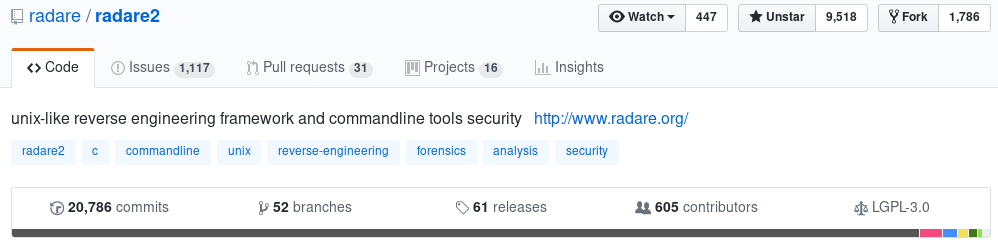
\includegraphics[width=\linewidth]{../medias/radare2-github.png}
  \begin{exampleblock}{Radare2 en quelques mots}
    \begin{itemize}
    \item{outil de reverse-engineering opensource (GPLv3)}
    \item{40+ architectures (x86, ARM, MIPS, SPARC...)}
    \item{30+ formats (ELF, PE, DEX...)}
    \item{écrit en C (bugs de corruption mémoire)}
    \item{20000+ commits, 600+ contributeurs, 900K+ LoC}
    \end{itemize}
  \end{exampleblock}
\end{frame}

%%%%%%%%%%%%%%%%%%%%%%%%%%%%%%%%%%%%%%%%%%%%%%%%%%%%%%%%%%%%%%%%%%%%%%%%%
% Présentation de la méthodologie
%%%%%%%%%%%%%%%%%%%%%%%%%%%%%%%%%%%%%%%%%%%%%%%%%%%%%%%%%%%%%%%%%%%%%%%%%
\begin{frame}[fragile]{Fuzzing de Radare2}{Méthodologie}
  \begin{block}{Méthodologie}
    \begin{itemize}
    \item{installation de AFL}
    \item{instrumentation de Radare2 grâce à \lstinline{afl-gcc}}
    \item{établir une base d'entrées initiales pour alimenter le fuzzer}
    \item{analyse des résultats avec Address Sanitizer}
    \end{itemize}
  \end{block}

  \pause

  \begin{exampleblock}{Récupération des sources}
    \begin{itemize}
    \item{\url{http://lcamtuf.coredump.cx/afl/releases/afl-latest.tgz}}
    \item{\url{https://github.com/radare/radare2}}
    \end{itemize}
  \end{exampleblock}

  \pause
  \vfill

  \begin{exampleblock}{Instrumentation de radare2}
    \begin{itemize}
    \item \lstinline{CC=afl-gcc ./sys/user.sh --install-path ../radare2-install}
    \end{itemize}
  \end{exampleblock}

\end{frame}


%%%%%%%%%%%%%%%%%%%%%%%%%%%%%%%%%%%%%%%%%%%%%%%%%%%%%%%%%%%%%%%%%%%%%%%%%
% Entrées de Radare2
%%%%%%%%%%%%%%%%%%%%%%%%%%%%%%%%%%%%%%%%%%%%%%%%%%%%%%%%%%%%%%%%%%%%%%%%%
\begin{frame}[fragile]{Fuzzing de Radare2}{Génération des entrées}
  \begin{center}
    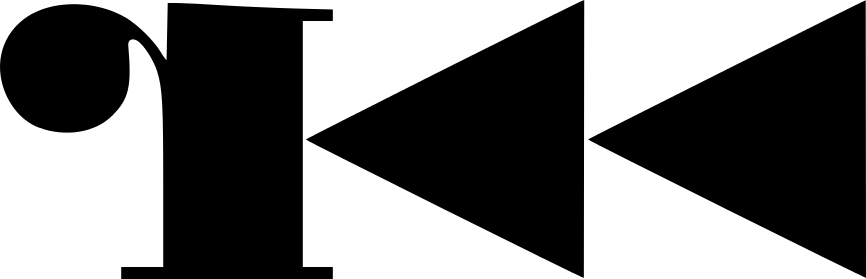
\includegraphics[width=0.25\textwidth, clip=true]{../medias/radare2-logo.png}
  \end{center}

  \begin{columns}[T]
    \begin{column}{0.44\linewidth}

      \begin{block}{Analyseur de fichiers}
        \begin{itemize}
        \item{\path{binary-samples/}}
        \item{\path{radare2-regressions/}}
        \item{sélection de petits binaires}
        \item{$\ne$ architectures/formats}
        \end{itemize}

        \vspace{1.75ex}
      \end{block}
    \end{column}

    \begin{column}{0.44\linewidth}
      \begin{block}{Interpréteur de commandes}
        \begin{itemize}
        \item{1 caractère = 1 action}
        \item{\lstinline{px} = ``Print hexdump''}
        \item{\lstinline{pxj} = ``Print hexdump in JSON''}
        \item{élaboration de scripts}
        \end{itemize}
      \end{block}
    \end{column}
  \end{columns}
  \pause
  \vfill
  \begin{exampleblock}{Autres outils}
    \begin{itemize}
    \item{\lstinline{rax2}, \lstinline{rabin2}, \lstinline{rafind2}, \lstinline{rasm2}, \lstinline{radiff2}, ...}
    \end{itemize}
  \end{exampleblock}
\end{frame}

%%%%%%%%%%%%%%%%%%%%%%%%%%%%%%%%%%%%%%%%%%%%%%%%%%%%%%%%%%%%%%%%%%%%%%%%%
% afl-fuzz en pratique
%%%%%%%%%%%%%%%%%%%%%%%%%%%%%%%%%%%%%%%%%%%%%%%%%%%%%%%%%%%%%%%%%%%%%%%%%
\begin{frame}{Fuzzing de Radare2}{afl-fuzz}
  \begin{figure}
    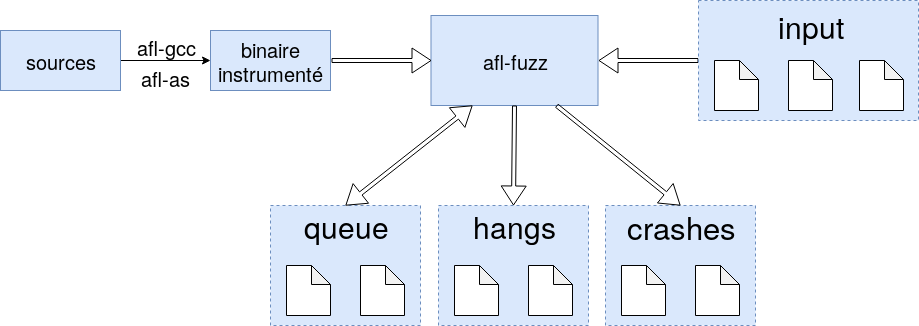
\includegraphics[width=0.98\linewidth]{../medias/afl-overview.png}
  \end{figure}

  \pause

  \begin{exampleblock}{afl-fuzz}
    \begin{itemize}
    \item{serveurs de calculs du CREMI : 48 CPU + 128 Go de RAM}
    \item{10 instances d'\lstinline{afl-fuzz}}
    \item{en tout, environ 1 semaine de fuzzing}
    \end{itemize}
  \end{exampleblock}

\end{frame}

\begin{frame}{Fuzzing de Radare2}{afl-fuzz}
  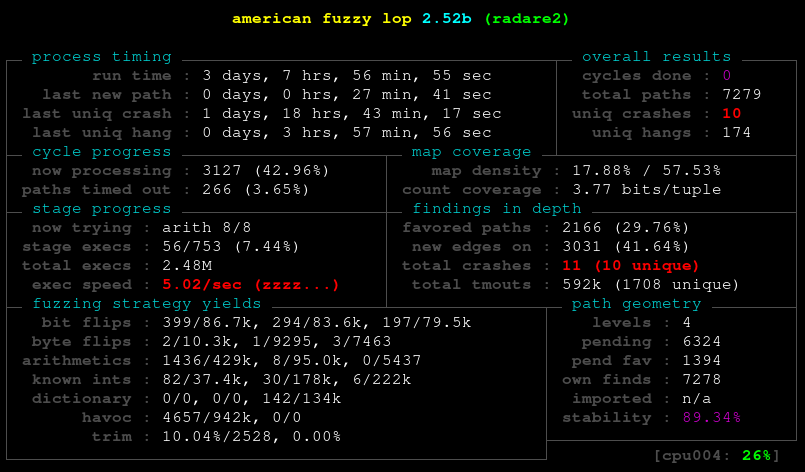
\includegraphics[width=\linewidth]{../medias/afl-fuzz.png}
\end{frame}

%%%%%%%%%%%%%%%%%%%%%%%%%%%%%%%%%%%%%%%%%%%%%%%%%%%%%%%%%%%%%%%%%%%%%%%%%
% Résultats
%%%%%%%%%%%%%%%%%%%%%%%%%%%%%%%%%%%%%%%%%%%%%%%%%%%%%%%%%%%%%%%%%%%%%%%%%
\begin{frame}{Fuzzing de Radare2}{Résultats}
  \begin{exampleblock}{Address Sanitizer (ASan)}
    \begin{itemize}
    \item{développé par Google}
    \item{instrumentation basée sur LLVM}
    \item{détecte certaines corruptions mémoires (overflows, UAF...)}
    \end{itemize}
  \end{exampleblock}

  \pause

  \begin{block}{Résultats}
    \begin{itemize}
    \item{10 bugs remontés et corrigés par Radare2}
    \item{3 read out-of-bounds}
    \item{2 double-free}
    \item{2 bad-pointer-dereference}
    \item{1 use-after-free}
    \item{1 stack-based-overflow}
    \item{1 integer-overflow}
    \end{itemize}
  \end{block}
\end{frame}

\section{Binaires quelconques et ciblant d'autres plateformes}

\begin{frame}{Binaires quelconques et ciblant d'autres plateformes}{Problème}
\end{frame}

\begin{frame}{Binaires quelconques et ciblant d'autres plateformes}{QEMU}
\end{frame}

\begin{frame}{Binaires quelconques et ciblant d'autres plateformes}{AFL avec le mode QEMU}
\end{frame}

\begin{frame}{Binaires quelconques et ciblant d'autres plateformes}{Autres versions d'AFL}
\end{frame}


\section*{Conclusion}

\begin{frame}{Conclusion}
  \begin{exampleblock}{Fuzzing "bête"}
    \begin{itemize}
      \item{ n'analyse pas du tout le programme pour générer des entrées}
      \item{trouve beaucoup de bugs en pratique}
      \item{exemples : AFL, peach, libfuzzer, ...}
    \end{itemize}
  \end{exampleblock}
  \begin{block}{Fuzzing "intelligent"}
    \begin{itemize}
      \item{peut utiliser de l'exécution symbolique}
      \item{pas très utilisable en pratique}
      \item{exemples : driller, manticore (trailofbits), ...}
    \end{itemize}
  \end{block}
\end{frame}

\begin{frame}{Conclusion}
  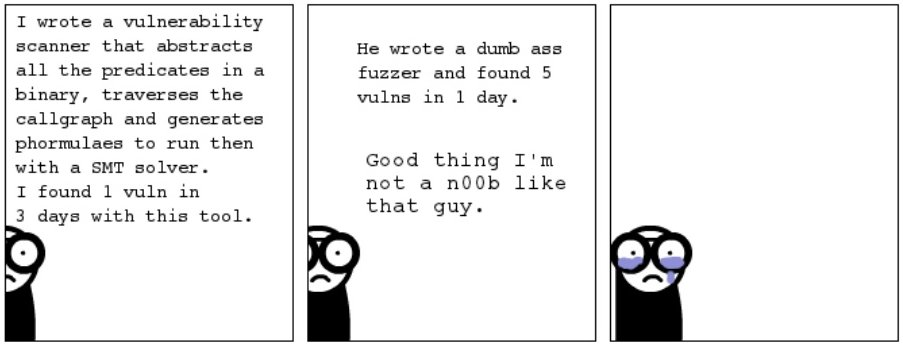
\includegraphics[width=\textwidth]{../medias/comics.png}
\end{frame}


\end{document}
